\newpage
\section{Application: Private and Compact Biometric Matching}
\label{sec:Application: Private and Compact Biometric Matching}

This section delves into the practical application of fuzzy hashing within the realm of biometric matching. Employing the Hamming distance for biometric matching offers a systematic approach by iteratively generating \textit{l} iterations of the preHash function, defined as:

\begin{equation}
    \begin{aligned}
        Hash_{key}^m &= Hash_{key_1, \ldots, key_l}^m(\bar{X})\\
        &= (preHash_{key_1}^m(\bar{X}), \ldots, preHash_{key_l}^m(\bar{X}))
    \end{aligned}
\end{equation}

Subsequently, the Hamming distance between the resulting hash values of two biometric samples \(X\) and \(Y\) is calculated as:

\begin{equation}
    \begin{aligned}
        \label{eq:HammingDist}
        d_H(Hash_{key}^m(\bar{X}), Hash_{key}^m(\bar{Y})) = \# \{i: preHash_{key_i}^m(\bar{X}) \neq preHash_{key_i}^m(\bar{Y})\}
    \end{aligned}
\end{equation}

This expression quantifies the instances "i" where the outputs of the preHash function differ between samples \(\bar{X}\) and \(\bar{Y}\).

One notable advantage of this approach is the reduction in size of the stored biometric template. Rather than storing \textit{n} pixels, \textit{ml} integers are stored. Additionally, the key renders the reference preHash less privacy-sensitive compared to a biometric template. Specifically, if the key is known, each integer in the hash discloses about \(\frac{1}{p}\) pixels, revealing \(\frac{ml}{p}\) pixels at worst. This disclosure occurs because, with the keys, the hash values can potentially be reverse-engineered to reveal characteristics of the original biometric pattern. The term \(p\)​ reflects the information entropy associated with each bit being a vein (\('1'\)) and thus quantifies the average information content each disclosed pixel conveys when the hash is decoded.

Similarly, when employing the Hamming distance for biometric matching through the iterative generation of \textit{l} iterations of the postHash function, analogous advantages arise. Here, the stored biometric template is condensed to \textit{mld} integers instead of \textit{n} pixels. Furthermore, the key diminishes the sensitivity of the reference postHash in terms of privacy, exposing \(\frac{mld}{p}\) pixels at most if known. Additionally, postHash contributes to leakage reduction.

It's crucial to note that for both scenarios, additional privacy safeguards can be implemented, for instance a restricted access to the key. Hence, the intricacies of the biometric infrastructure must be addressed on a case-by-case basis.

\subsection{Theoretical Foundations of FPR and FNR within Fuzzy Hashing Systems}

Transforming biometric data into a hash, using methods such as preHash or its more compact version, postHash, plays a key role in enhancing the system's efficiency and security. This process helps protect privacy, which in turn influences important aspects of the system's performance, such as the \hyperref[def:FNR]{False Negative Rate (FNR)} and the \hyperref[def:FPR]{False Positive Rate (FPR)}. By converting detailed biometric data into a simpler, hashed format, the system not only uses storage space more efficiently but also reduces the chances of unauthorized access to sensitive information. This transformation is crucial for maintaining the integrity of the data and provides a strong line of defense against potential security threats. Additionally, choosing the right techniques for generating these hashes can greatly improve the system's ability to distinguish between authorized and unauthorized users. This means fewer mistakes in the form of false rejections or acceptances, leading to a more accurate and dependable biometric verification process.

We establish a threshold \(t\) to evaluate the match between two biometric samples, \(\bar{X}\) and \(\bar{Y}\), by analyzing the Hamming distance between their hash values.
We define that a match is confirmed if the difference between \(l\) (the total iterations) and the Hamming distance is equal to or exceeds the threshold \(t\), expressed as: \[l - d_H(Hash_{key}^m(\bar{X}), Hash_{key}^m(\bar{Y})) \geq t\]
In contrast, we define there being no match if the following equation holds: \[l - d_H(Hash_{key}^m(\bar{X}), Hash_{key}^m(\bar{Y})) < t\]

To further refine our understanding, we use statistical methods to approximate this comparison to a normal distribution, allowing us to more accurately calculate the False Negative Rate (FNR). 

First, let us define the random variable $H$ as \(H = d_H(Hash_{key}^m(\bar{X}), Hash_{key}^m(\bar{Y}))\), representing the number of positions where the preHash values of two samples differ, capturing the number of keys with different hashes. Supposing that the hash keys are generated such that each preHash comparison is independent, the Hamming distance $H$ can be modeled as a binomial random variable, \(H \sim Binomial(l, p_H)\), where $l$ is the total number of iterations and $p_H = Pr[Hash_{key_i}^m(\bar{X}) \neq Hash_{key_i}^m(\bar{Y})] = 1 - \mu_{\text{same}}^m$ is the probability that the output of the preHash function for a certain key mismatches. This probability uses $\mu_{\text{same}}$ because we are approximating the FNR, which, by definition, is when the samples should match but don't. 
\newline For a large $l$, the binomial distribution can be approximated by a normal distribution using the Central Limit Theorem. The mean and variance of the binomial distribution are given by
\[
\mu_{\text{H, same}} = \mathbb{E}(H) = l \cdot p_H = l \cdot (1 - \mu_{\text{same}}^m)    
\]
\[
\sigma_{\text{H, same}}^2 = \mathbb{V}(H) = l \cdot p_H \cdot (1 - p_H) = l \cdot (1 - \mu_{\text{same}}^m) \cdot \mu_{\text{same}}^m   
\]
Therefore, H can be approximated by
\[
H \sim \mathcal{N}(\mu_{\text{H, same}}, \sigma_{\text{H, same}}^2)    
\]
The FNR is the probability that the Hamming distance $H$ exceeds $l - t$ in cases where there should be a match. This is given by
\begin{equation}
    \begin{aligned}
        \label{eq:fnr}
        FNR &= Pr[l - H < t] = Pr[H > l - t] \\
        &= Pr\left[\frac{H - \mu_{\text{H, same}}}{\sigma_{\text{H, same}}} > \frac{l - t - \mu_{\text{H, same}}}{\sigma_{\text{H, same}}}\right] \\
        &= \Phi \left( - \frac{l - t - \mu_{\text{H, same}}}{\sigma_{\text{H, same}}}\right) \\
        &= \Phi \left(\frac{t - l\mu_{\text{same}}}{\sqrt{l \cdot (1 - \mu_{\text{same}}^m) \cdot \mu_{\text{same}}^m}}\right) \\
        &\approx \Phi \left(\frac{t - l\mu_{\text{same}}}{\sqrt{l\mu_{\text{same}}^m}}\right) \\
    \end{aligned}        
\end{equation}
where the last equality is obtained because $l\cdot(\mu_{\text{same}}^m)^2$ is negligeable. 

Here, \(\Phi\) denotes the Cumulative Distribution Function (CDF) of the standard normal distribution, denoted as \(\mathcal{N}(0, 1)\).

Using the same deduction as the previous paragraph and considering that for the False Positive Rate (FPR) we use \(\mu_{\text{diff}}\) instead of \(\mu_{\text{same}}\), we can derive the FPR as follows. The FPR is the probability that non-matching biometric samples are incorrectly identified as matches by the system. 

Let \( H \) represent the Hamming distance as before. When dealing with non-matching samples, the probability of a mismatch for any given preHash iteration is denoted by \( \mu_{\text{diff}} \). Thus, the probability of a mismatch is \( p_H = 1 - \mu_{\text{diff}}^m \).

For a large \( l \), the Hamming distance \( H \) can again be approximated by a normal distribution. The mean and variance for the non-matching case are given by:
\[
\mu_{\text{H, diff}} = l \cdot (1 - \mu_{\text{diff}}^m)
\]
\[
\sigma_{\text{H, diff}}^2 = l \cdot (1 - \mu_{\text{diff}}^m) \cdot \mu_{\text{diff}}^m
\]

Therefore, \( H \) can be approximated by:
\[
H \sim \mathcal{N}(\mu_{H, \text{diff}}, \sigma_{H, \text{diff}}^2)
\]

The FPR is the probability that the Hamming distance \( H \) is less than the threshold \( l - t \) in cases where the samples should not match. This is given by:
\begin{equation}
\begin{aligned}
    \label{eq:fpr}
    \text{FPR} &= Pr[H \leq l - t] \\
    &= Pr\left[\frac{H - \mu_{H, \text{diff}}}{\sigma_{H, \text{diff}}} \leq \frac{l - t - \mu_{H, \text{diff}}}{\sigma_{H, \text{diff}}}\right] \\
    &= \Phi\left(\frac{l - t - \mu_{H, \text{diff}}}{\sigma_{H, \text{diff}}}\right) \\
    &= \Phi\left(-\frac{t - l\mu_{\text{diff}}^m}{\sqrt{l \cdot (1 - \mu_{\text{diff}}^m) \cdot \mu_{\text{diff}}^m}}\right)\\
    &\approx\Phi\left(-\frac{t - l\mu_{\text{diff}}^m}{\sqrt{l\cdot \mu_{\text{diff}}^m}}\right)
\end{aligned}
\end{equation}

These formulations allow for the evaluation of false match rates based on the standard deviation and mean of the distributions for same and different samples, respectively.e

For instance, employing \(\Phi(-2.33) \approx 1\%\) as a benchmark, we calculate the threshold (\(t\)) from parameters \(m\) and \(l\) to achieve an FNR of \(\approx\) 1\%. The theoretical resulting set of parameters is as follows: 

\begin{table}[htbp] 
    \centering
    \begin{tabular}{|c|c|c|c|c|c|c|}
        \hline
        \textit{m} & \textit{l} & \textit{t} & \textit{l}\(\mu_{\text{same}}^m\) & \textit{l}\(\mu_{\text{diff}}^m\) & \textit{FNR} & \textit{FPR} \\
        \hline
        1 & 217 & 32 & 47.85 & 17.9 & \(\leq\)1\% & \(2^{-10}\)\\
        1 & 637 & 113 & 140.46 & 52.55 & 1.0\% & \(2^{-54}\) \\
        %1 & 637 & 118 & 146.5 & 49 & 2^⁻6\% & \(2^{-74}\) \\
        2 & 961 & 31 & 46.72 & 6.54 & 1.0\% & \(2^{-69}\) \\
        %2 & 961 & 34 & 50.8 & 5.7 & 2^⁻6\% & \(2^⁻106\) \\
        3 & 2569 & 15 & 27.54 & 1.44 & 1.0\% &\(2^{-101}\) \\
        \hline
    \end{tabular}
    \caption{Theoretical Parameterization Results for FNR and FPR Calculation, using $l$ Iterations of PreHash}
    \label{tab:theoretical_parameterization_PreHash}
\end{table}

Using compression techniques implemented through postHash, specifically compressing to \( D = 16 \) (\( d = 4 \)) and \( D = 2 \) (\( d = 1 \)), we calculate the threshold (\( t \)) from parameters \( m = 1 \) and \( l \) to achieve an FNR of \(\approx\) \(1\%\). The introduction of compression slightly modifies the equations for FNR (\ref{eq:fnr}) and FPR (\ref{eq:fpr}), necessitating the use of \( q \) in place of \(\mu^m\). The theoretical resulting set of parameters is as follows:

\begin{table}[htbp] 
    \centering
    \begin{tabular}{|c|c|c|c|c|c|c|c|}
        \hline
        \textit{m} & \textit{d} & \textit{l} & \textit{t} & \textit{l}\(q_{\text{same}}^m\) & \textit{l}\(q_{\text{diff}}^m\) & \textit{FNR} & \textit{FPR} \\
        \hline
        1 & 4 & 1107 & 258 & 298 & 145.3 & 1.0\% & \(2^{-67}\) \\
        1 & 4 & 347 & 71 & 93.4 & 45.6 & \(\leq\)1.0\% & \(2^{-13}\)\\
        1 & 1 & 3597 & 2104 & 2213.2 & 1895.3 & \(\leq\)1.0\% & \(2^{-20}\)\\
        \hline
    \end{tabular}
    \caption{Theoretical Parameterization Results for FNR and FPR Calculation, using $l$ Iterations of PostHash}
    \label{tab:theoretical_parameterization_PostHash}
\end{table}


\newpage
\subsection{Experimental Derivation of the FNR and FPR for Different (\(m, l\)) Parameter Configurations}

To experimentally determine the False Negative Rate (FNR) and the False Positive Rate (FPR) for various \((m, l)\) parameter configurations, the initial step is to compute the Hamming distance between \( Hash_{\text{key}}^m(\bar{X}) \) and \( Hash_{\text{key}}^m(\bar{Y}) \). The \( Hash_{\text{key}}^m \) of an extracted feature vector is generated using \( l \) iterations of preHash. We designed an algorithm that accepts a list of \( l \) keys (since each preHash iteration requires a new key) and the parameter \( m \), which indicates the number of indices each call to preHash should generate per key. For testing purposes, the \( l \) keys are simply integers from 0 to \( l-1 \), converted into a two-byte binary format. We then calculate the Hamming distance between the resulting hash values for pairs of images. The Hamming distance between \( Hash_{\text{key}}^m(\bar{X}) \) and \( Hash_{\text{key}}^m(\bar{Y}) \) is defined as the number of positions at which the corresponding iterations of preHash are different, as defined in Equation \ref{eq:HammingDist}. In this formula, the expression \( \# \{ i : preHash_{\text{key}_i}^m(\bar{X}) \neq preHash_{\text{key}_i}^m(\bar{Y}) \} \) counts the number of iterations \( i \) where the pre-hash values of \( \bar{X} \) and \( \bar{Y} \) differ. Each comparison results in a \(1\) if the iterations differ and a \(0\) if they are the same. Summing these comparison results gives the total number of differing positions, thereby computing the Hamming distance between the hash values of the iterations.


Each experiment we conducted uses a different row from Table \ref{tab:theoretical_parameterization_PreHash}. In each experiment, we generate \( l \) preHash iterations for all image pairs and then determine if two images, \(\bar{X}\) and \(\bar{Y}\), are a match, defined as \( l - d_H(Hash_{\text{key}}^m(\bar{X}), Hash_{\text{key}}^m(\bar{Y})) \geq t \). We perform two types of comparisons on our data:


\begin{enumerate}
    \item \textbf{Same Person, Same Finger Comparisons}: This involves comparing different trials of images from the same person and the same finger. These comparisons should theoretically result in a match. If two such images do not match (i.e., \( l - d_H(Hash_{\text{key}}^m(\bar{X}), Hash_{\text{key}}^m(\bar{Y})) < t \)), this contributes to the FNR.
    \item \textbf{Different People or Fingers Comparisons}: This involves comparing images from different people and/or different fingers. These comparisons should theoretically not result in a match. If two such images do match, this contributes to the FPR.
\end{enumerate}

To calculate the False Negative Rate (FNR), we count the instances where images that should match do not, and then compute the mean of these instances. Similarly, for the False Positive Rate (FPR), we count the instances where images that should not match do, and then compute the mean of these instances.

For the experiments from Table \ref{tab:theoretical_parameterization_PreHash}, we obtain the following results:

\begin{enumerate}
    \item \textbf{m = 1, l = 217 and t = 32}
        \begin{itemize}
            \item $FNR = 18.91\%$
            \item $FPR = 2^{-9}$

            \begin{figure}[H]
                \centering
                \begin{minipage}[b]{0.48\linewidth}
                    \centering
                    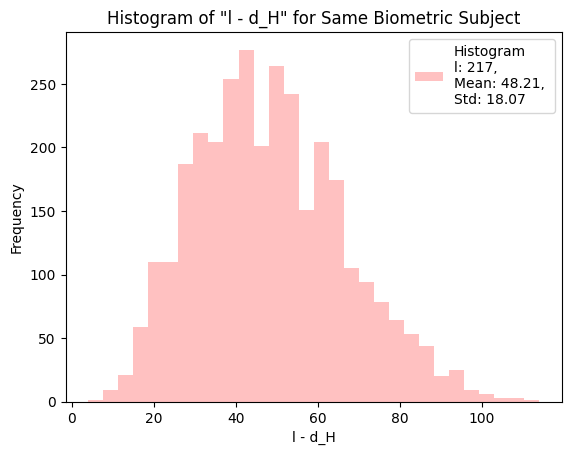
\includegraphics[width=\linewidth,height=7cm,keepaspectratio]{latex-img/l-dHconfig1a_same.png}
                    \caption{Distribution of the Difference between the Total Number of Iterations and the Hamming Distance between Pairs of Same, Aligned Biometric Samples with Single Index PreHashing and $217$ Total Number of Iterations}
                    \label{l-dHconfig1a_same}
                \end{minipage}
                \hfill
                \begin{minipage}[b]{0.48\linewidth}
                    \centering
                    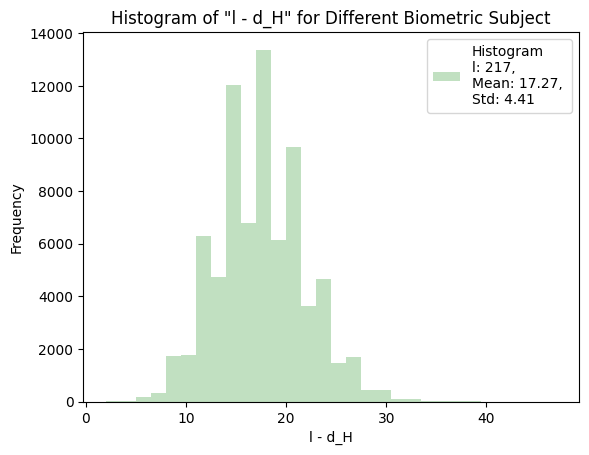
\includegraphics[width=\linewidth,height=7cm,keepaspectratio]{latex-img/l-dHconfig1a_diff.png}
                    \caption{Distribution of the Difference between the Total Number of Iterations and the the Hamming Distance between Pairs of Different, Aligned Biometric Samples with Single Index PreHashing and $217$ Total Number of Iterations}
                    \label{l-dHconfig1a_diff}
                \end{minipage}
            \end{figure}
            
            \begin{figure}[H]
                \centering
                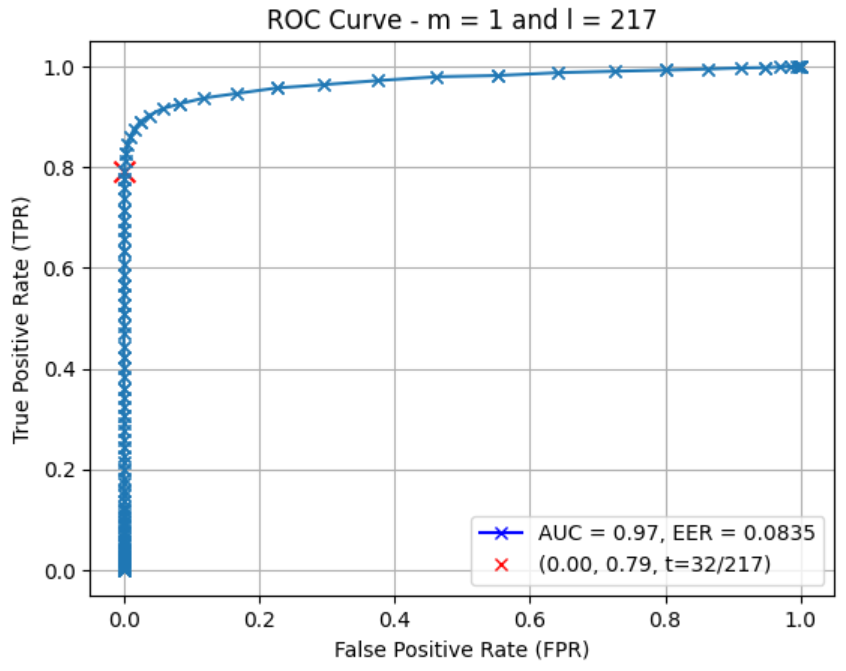
\includegraphics[width=\linewidth,height=8.5cm,keepaspectratio]{latex-img/FNR-FPR_ROC_TPR_config1a.png}
                \caption{ROC for (m = 1, l = 217)}
                \label{FNR-FPR_ROC_TPR_config1a}
            \end{figure}
        \end{itemize}
                    
    \item \textbf{m = 1, l = 637 and t = 113}
        \begin{itemize}
            \item $FNR = 31.75\%$
            \item $FPR = 2^{-14}$ 

            \begin{figure}[H]
                \centering
                \begin{minipage}[b]{0.48\linewidth}
                    \centering
                    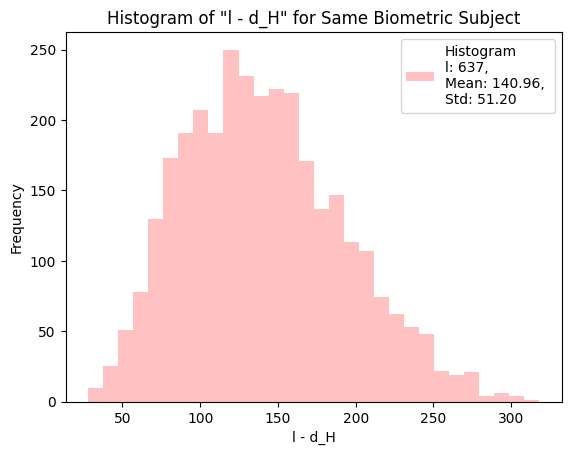
\includegraphics[width=\linewidth,height=7cm,keepaspectratio]{latex-img/l-dHconfig1_same.png}
                    \caption{Distribution of the Difference between the Total Number of Iterations and the Hamming Distance between Pairs of Same, Aligned Biometric Samples with Single Index PreHashing and $637$ Total Number of Iterations}
                    \label{l-dHconfig1_same}
                \end{minipage}
                \hfill
                \begin{minipage}[b]{0.48\linewidth}
                    \centering
                    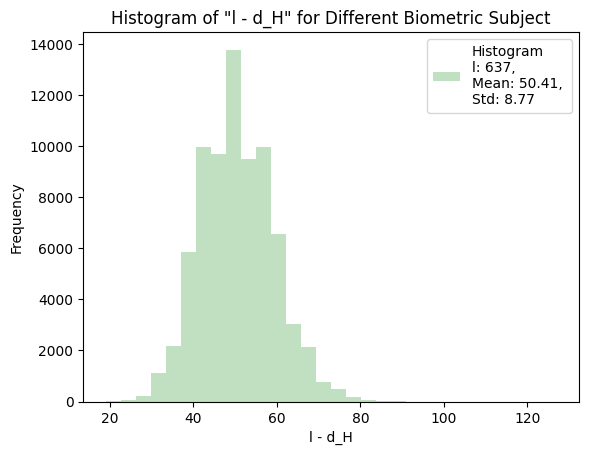
\includegraphics[width=\linewidth,height=7cm,keepaspectratio]{latex-img/l-dHconfig1_diff.png}
                    \caption{Distribution of the Difference between the Total Number of Iterations and the Hamming Distance between Pairs of Different, Aligned Biometric Samples with Single Index PreHashing and $637$ Total Number of Iterations}
                    \label{l-dHconfig1_diff}
                \end{minipage}
            \end{figure}

            \begin{figure}[H]
                \centering
                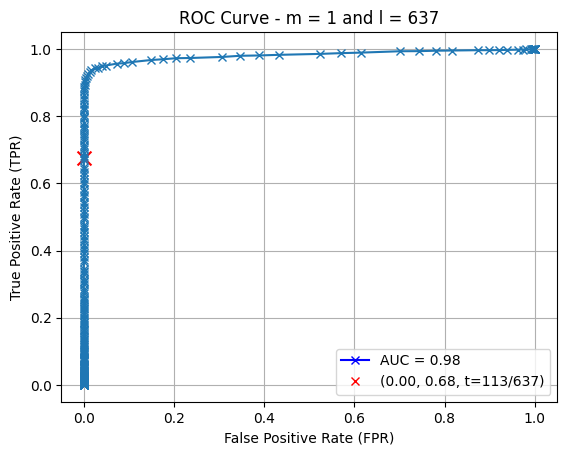
\includegraphics[width=\linewidth,height=8.5cm,keepaspectratio]{latex-img/FNR-FPR_ROC_TPR_config1.png}
                \caption{ROC for (m = 1, l = 637)}
                \label{FNR-FPR_ROC_TPR_config1}
            \end{figure}
        \end{itemize}
    \item \textbf{m = 2, l = 961 and t = 31}
        \begin{itemize}
            \item  $FNR = 33.32\%$
            \item $FPR = 2^{-14}$

            \begin{figure}[H]
                \centering
                \begin{minipage}[b]{0.48\linewidth}
                    \centering
                    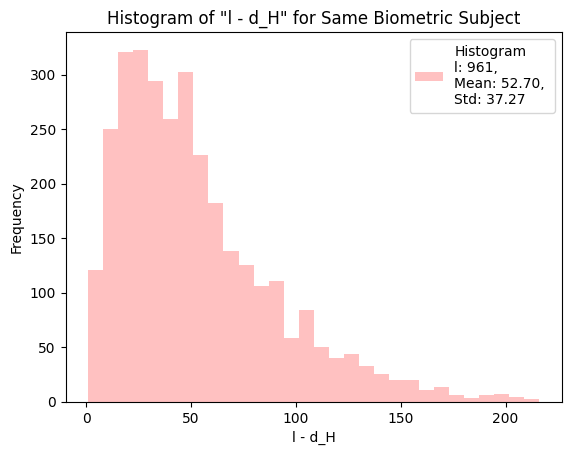
\includegraphics[width=\linewidth,height=7cm,keepaspectratio]{latex-img/l-dHconfig2_same.png}
                    \caption{Distribution of the Difference between the Total Number of Iterations and the Hamming Distance between Pairs of Same, Aligned Biometric Samples with Double Index PreHashing and $961$ Total Number of Iterations}
                    \label{l-dHconfig2_same}
                \end{minipage}
                \hfill
                \begin{minipage}[b]{0.48\linewidth}
                    \centering
                    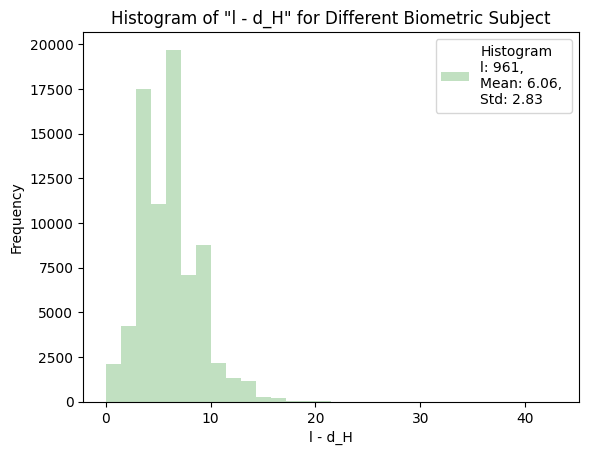
\includegraphics[width=\linewidth,height=7cm,keepaspectratio]{latex-img/l-dHconfig2_diff.png}
                    \caption{Distribution of the Difference between the Total Number of Iterations and the Hamming Distance between Pairs of Different, Aligned Biometric Samples with Double Index PreHashing and $961$ Total Number of Iterations}
                    \label{l-dHconfig2_diff}
                \end{minipage}
            \end{figure}

            \begin{figure}[H]
                \centering
                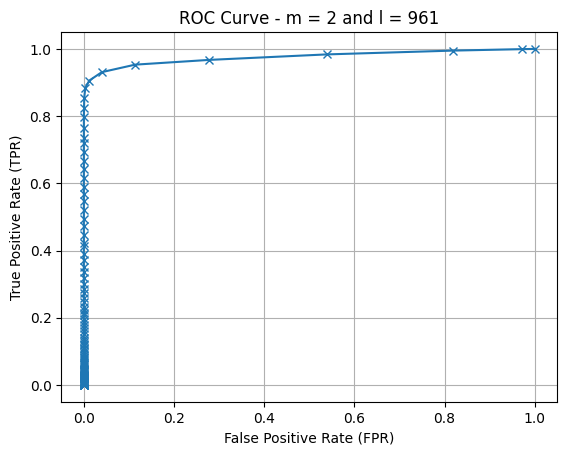
\includegraphics[width=\linewidth,height=8.5cm,keepaspectratio]{latex-img/FNR-FPR_ROC_TPR_config2.png}
                \caption{ROC for (m = 2, l = 961)}
                \label{FNR-FPR_ROC_TPR_config2}
            \end{figure}
        \end{itemize}
    \item \textbf{m = 3, l = 2'569 and t = 15}
        \begin{itemize}
            \item $FNR = 33.45\%$
            \item $FPR = 2^{-13}$ 

            \begin{figure}[H]
                \centering
                \begin{minipage}[b]{0.48\linewidth}
                    \centering
                    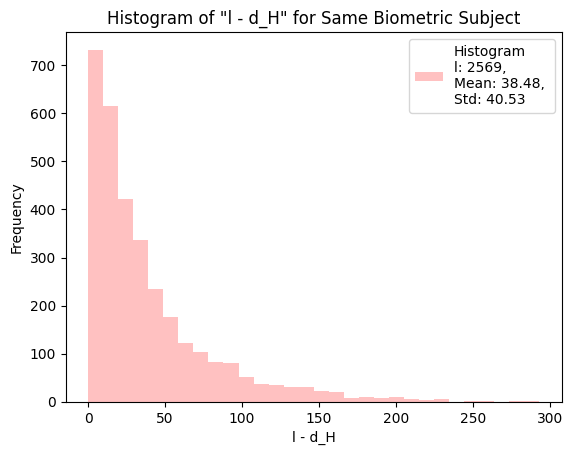
\includegraphics[width=\linewidth,height=7cm,keepaspectratio]{latex-img/l-dHconfig3_same.png}
                    \caption{Distribution of the Difference between the Total Number of Iterations and the Hamming Distance between Pairs of Same, Aligned Biometric Samples with Triple Index PreHashing and $2'569$ Total Number of Iterations}
                    \label{l-dHconfig3_same}
                \end{minipage}
                \hfill
                \begin{minipage}[b]{0.48\linewidth}
                    \centering
                    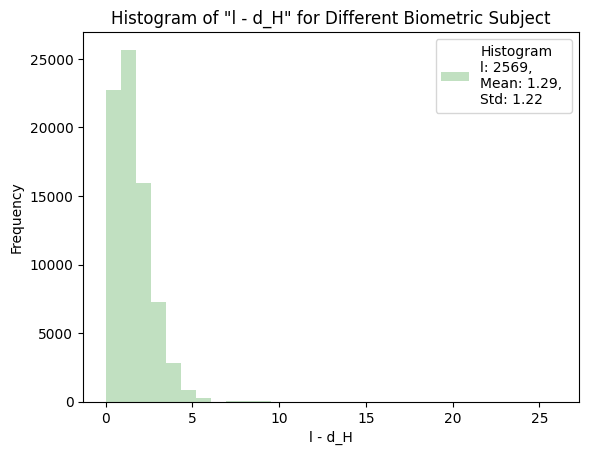
\includegraphics[width=\linewidth,height=7cm,keepaspectratio]{latex-img/l-dHconfig3_diff.png}
                    \caption{Distribution of the Difference between the Total Number of Iterations and the Hamming Distance between Pairs of Different, Aligned Biometric Samples with Triple Index PreHashing and $2'569$ Total Number of Iterations}
                    \label{l-dHconfig3_diff}
                \end{minipage}
            \end{figure}

            \begin{figure}[H]
                    \centering
                    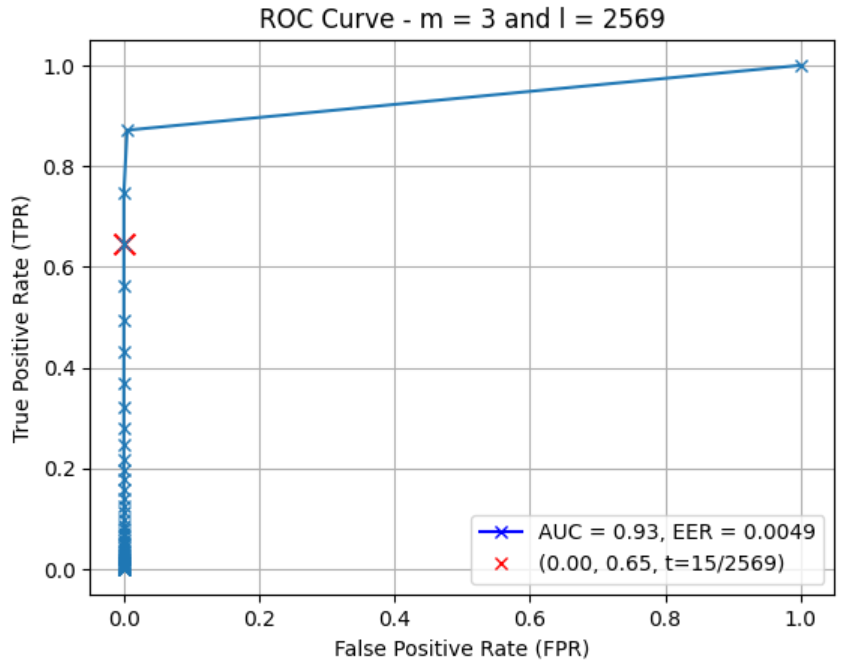
\includegraphics[width=\linewidth,height=8.5cm,keepaspectratio]{latex-img/FNR-FPR_ROC_TPR_config3.png}
                    \caption{ROC for (m = 3, l = 2'569)}
                    \label{FNR-FPR_ROC_TPR_config3}
            \end{figure}
        \end{itemize}
\end{enumerate}

From all figures in this subsection, we observe that the experimental means of the distributions for same and different biometric samples closely align with the theoretical means predicted (\(l\cdot\mu_{\text{same/diff}}^m\)) as shown in Table \ref{tab:theoretical_parameterization_PreHash}. Additionally, the experimental standard deviations of the distributions for different biometric samples are relatively close to the theoretically deduced values, defined as \(\sqrt{l\cdot\mu_{\text{diff}}^m}\). However, the standard deviations of the distributions for same biometric samples are significantly larger than the predicted values, which explains why the histograms of these distributions deviate from the predicted Normal Distribution. This discrepancy could be due to the incorrect assumption that the random variable \(H\) follows a Binomial distribution. 

It is possible that the assumption of independence among the \(l\) hash comparisons generated with their respective keys was incorrect. This dependence might be explained by the consistent identification of areas in the feature vector where vein concentration is higher or lower across all images. Such non-uniformity in the vein patterns could lead to correlations between hash comparisons that violate the independence assumption. Furthermore, we suppose that for two keys to define independent pairs of hashes, the two sequences of indices they define should not have overlapping elements located too far forward. If they do, the probability that \( Hash_{key_{i+1}}^m(\bar{X}) = Hash_{key_{i+1}}^m(\bar{Y}) \) given \( Hash_{key_{i}}^m(\bar{X}) = Hash_{key_{i}}^m(\bar{Y}) \) is higher than the probability that \( Hash_{key_{i+1}}^m(\bar{X}) = Hash_{key_{i+1}}^m(\bar{Y}) \)
alone. This might explain the observed dependencies and larger standard deviations.

Further analysis of the variance of the Hamming distances normalized by \( l \) (i.e., \(\mathbb{V}(H) / l\)) across different configurations suggests that this ratio does not behave as a constant. For example, in our experiments, this ratio varied significantly for both same and different biometric samples. Specifically, for same biometric samples, the ratio decreased from 4.1152 to 0.6394 as \( l \) increased from 217 to 2569. Similarly, for different biometric samples, the ratio decreased from 0.1209 to 0.0006 over the same range of \( l \). This indicates a complex relationship between \( l \) and the variance of Hamming distances, as observed in Figure \ref{variance_iterations}. It is important to note that the number of experiments conducted to plot this figure is insufficient to accurately determine the exact nature of this variance, and thus these results should be interpreted with caution.

\begin{figure}[H]
    \centering
    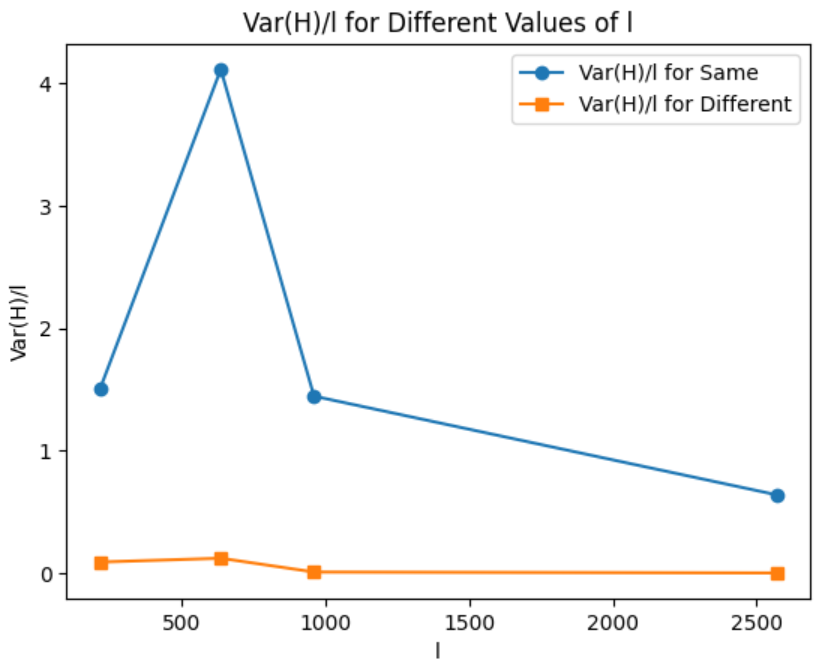
\includegraphics[width=\linewidth,height=7cm,keepaspectratio]{latex-img/variance_iterations.png}
    \caption{Ratio \(\frac{\mathbb{V}(H)}{l}\) for both 'Same' and 'Different' biometric samples}
    \label{variance_iterations}
\end{figure}

Furthermore, the ROC curves plotted in this section provide valuable insights into the system's performance across different parameter configurations. These curves illustrate the trade-off between the False Positive Rate (FPR) and True Positive Rate (TPR) at various threshold settings. Although the area under the curve (AUC) values of our ROC curves are close to 1, indicating a generally strong performance, the system's overall effectiveness is compromised by high False Negative Rate (FNR) values. This is evident from the plots, where achieving a low FPR does not correspond with a TPR close to 1, resulting in an undesirably high FNR (FNR = 1 - TPR). Evaluating whether the system is optimal depends on the specific real-world application and its tolerance for false positives and false negatives. For applications requiring high security, a lower FPR might be prioritized, even at the expense of a higher FNR. Conversely, for applications where user convenience is critical, a higher TPR might be favored, accepting a slightly higher FPR. This underscores the necessity of tuning the system parameters to strike an appropriate balance based on the intended use case.

Interestingly, we observe that increasing \(m\) and, more specifically, \(l\), does not necessarily lead to a better FPR. In some configurations, more iterations do not improve the system's ability to correctly identify different biometric samples, indicating that simply increasing the number of hash comparisons may not enhance performance as expected. In our experiments, while some configurations with higher \(l\) showed ROC curves closer to the top-left corner, indicating better performance with lower FPRs and higher TPR's, others did not. This variability suggests that there is a complex relationship between the number of iterations and the system's performance metrics.

\subsection{Experimental Derivation of the FNR and FPR for Different (\(m, l, d\)) Parameter Configurations with Compression}

In this subsection, we will experimentally evaluate the False Negative Rate (FNR) and False Positive Rate (FPR) with compression. We designed an algorithm that uses the previously defined method to generate \( l \) iterations of preHash and then compresses each hash value generated depending on the value of \(D = 2^d\). For an image, the algorithm generates a list of the \( l \) iterations of preHash and then applies the postHash algorithm to each preHash output.

After both images pass through this process, each iteration of each image is compared, resulting in a 1 if the iterations differ and a 0 if they are the same. Summing these comparison results gives the total number of ones, effectively computing the Hamming distance between the compressed and hashed images.

\begin{enumerate}
    \item \textbf{d = 4, m = 1, l = 1'107 and t = 258}
        \begin{itemize}
            \item $FNR = 39.76\%$
            \item $FPR = 2^{-15}$

            \begin{figure}[H]
                \centering
                \begin{minipage}[b]{0.48\linewidth}
                    \centering
                    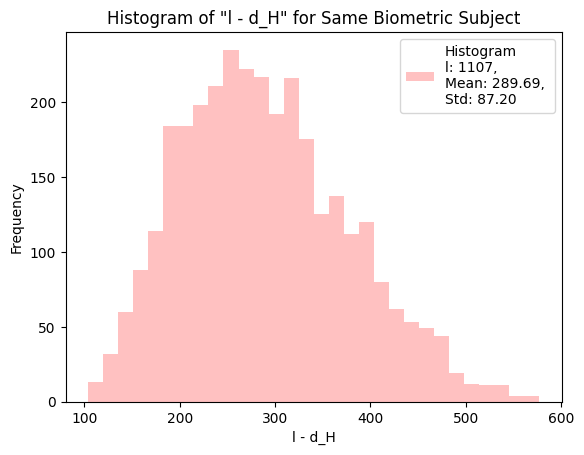
\includegraphics[width=\linewidth,height=7cm,keepaspectratio]{latex-img/l-dHconfig1_same_compression.png}
                    \caption{Distribution of the Difference between the Total Number of Iterations and the Hamming Distance between Pairs of Same, Aligned Biometric Samples with Single Index PreHashing, Hexadecimal PostHash Compression and $1'107$ Total Number of Iterations}
                    \label{l-dHconfig1a_same}
                \end{minipage}
                \hfill
                \begin{minipage}[b]{0.48\linewidth}
                    \centering
                    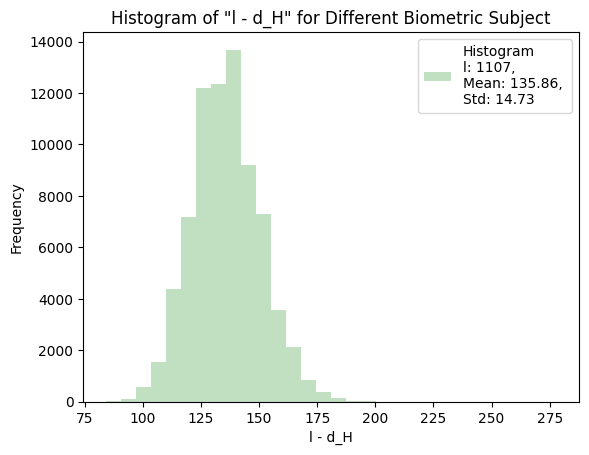
\includegraphics[width=\linewidth,height=7cm,keepaspectratio]{latex-img/l-dHconfig1_diff_compression.png}
                    \caption{Distribution of the Difference between the Total Number of Iterations and the the Hamming Distance between Pairs of Different, Aligned Biometric Samples with Single Index PreHashing, Hexadecimal PostHash Compression and $1'107$ Total Number of Iterations}
                    \label{l-dHconfig1a_diff}
                \end{minipage}
            \end{figure}
            
            \begin{figure}[H]
                \centering
                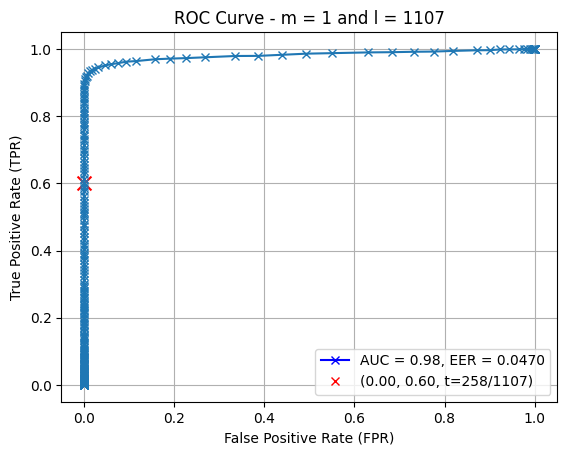
\includegraphics[width=\linewidth,height=8.5cm,keepaspectratio]{latex-img/FNR-FPR_ROC_config1_compression.png}
                \caption{ROC for (d = 4, m = 1, l = 1'107)}
                \label{FNR-FPR_ROC_TPR_config1a}
            \end{figure}
        \end{itemize}
                    
    \item \textbf{d = 4, m = 1, l = 347 and t = 71}
        \begin{itemize}
            \item $FNR = 25.69\%$
            \item $FPR = 2^{-11}$  

            \begin{figure}[H]
                \centering
                \begin{minipage}[b]{0.48\linewidth}
                    \centering
                    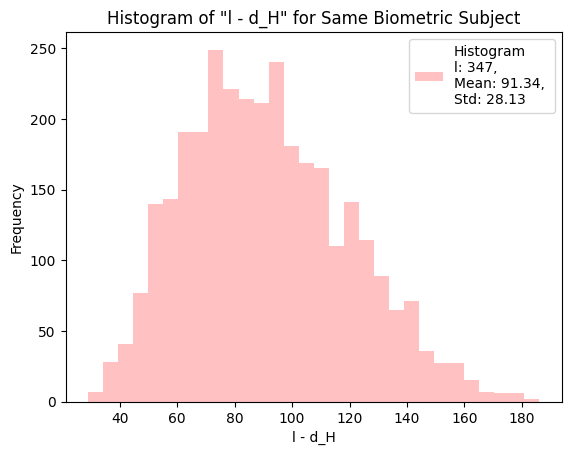
\includegraphics[width=\linewidth,height=7cm,keepaspectratio]{latex-img/l-dHconfig2_same_compression.png}
                    \caption{Distribution of the Difference between the Total Number of Iterations and the Hamming Distance between Pairs of Same, Aligned Biometric Samples with Single Index PreHashing, Hexadecimal PostHash Compression and $347$ Total Number of Iterations}
                    \label{l-dHconfig1_same}
                \end{minipage}
                \hfill
                \begin{minipage}[b]{0.48\linewidth}
                    \centering
                    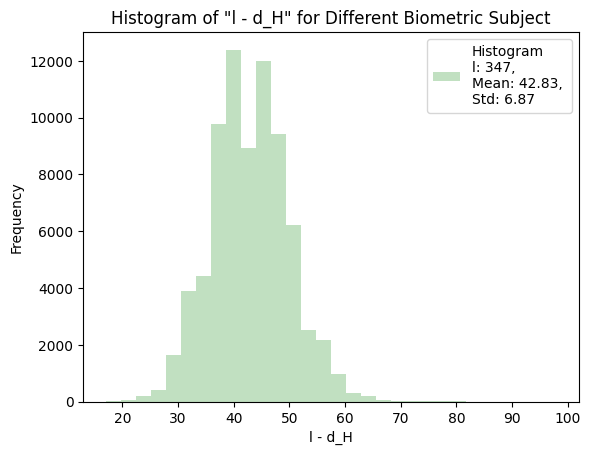
\includegraphics[width=\linewidth,height=7cm,keepaspectratio]{latex-img/l-dHconfig2_diff_compression.png}
                    \caption{Distribution of the Difference between the Total Number of Iterations and the Hamming Distance between Pairs of Different, Aligned Biometric Samples with Single Index PreHashing, Hexadecimal PostHash Compression and $347$ Total Number of Iterations}
                    \label{l-dHconfig1_diff}
                \end{minipage}
            \end{figure}

            \begin{figure}[H]
                \centering
                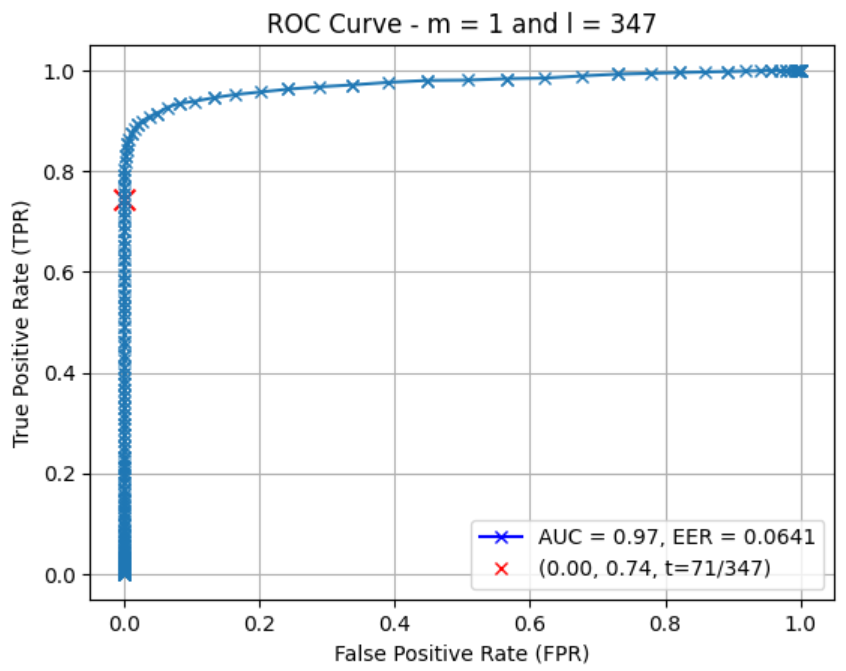
\includegraphics[width=\linewidth,height=8.5cm,keepaspectratio]{latex-img/FNR-FPR_ROC_config2_compression.png}
                \caption{ROC for (d = 4, m = 1, l = 347)}
                \label{FNR-FPR_ROC_TPR_config1}
            \end{figure}
        \end{itemize}
    \item \textbf{d = 1, m = 1, l = 3'597 and t = 2'104}
        \begin{itemize}
            \item  $FNR = 16.83\%$
            \item $FPR = 2^{-9}$

            \begin{figure}[H]
                \centering
                \begin{minipage}[b]{0.48\linewidth}
                    \centering
                    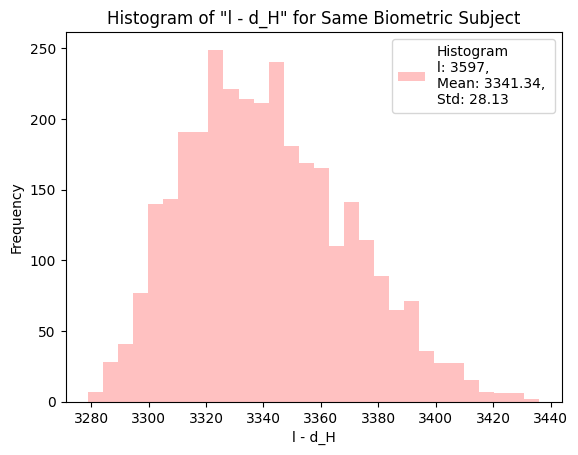
\includegraphics[width=\linewidth,height=7cm,keepaspectratio]{latex-img/l-dHconfig3_same_compression.png}
                    \caption{Distribution of the Difference between the Total Number of Iterations and the Hamming Distance between Pairs of Same, Aligned Biometric Samples with Double Index PreHashing, Binary PostHash Compression and $3'597$ Total Number of Iterations}
                    \label{l-dHconfig2_same}
                \end{minipage}
                \hfill
                \begin{minipage}[b]{0.48\linewidth}
                    \centering
                    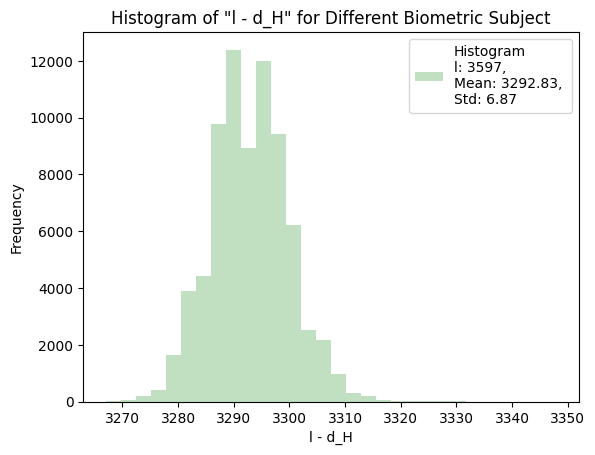
\includegraphics[width=\linewidth,height=7cm,keepaspectratio]{latex-img/l-dHconfig3_diff_compression.png}
                    \caption{Distribution of the Difference between the Total Number of Iterations and the Hamming Distance between Pairs of Different, Aligned Biometric Samples with Double Index PreHashing, Binary PostHash Compression and $3'597$ Total Number of Iterations}
                    \label{l-dHconfig2_diff}
                \end{minipage}
            \end{figure}

            \begin{figure}[H]
                \centering
                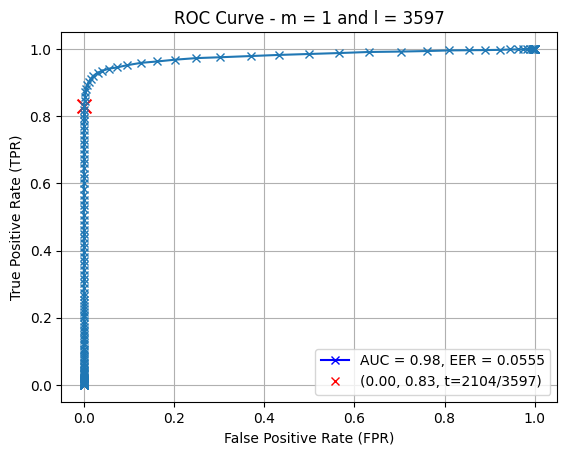
\includegraphics[width=\linewidth,height=8.5cm,keepaspectratio]{latex-img/FNR-FPR_ROC_config3_compression.png}
                \caption{ROC for (d = 1, m = 1, l = 3'597)}
                \label{FNR-FPR_ROC_TPR_config2}
            \end{figure}
        \end{itemize}
\end{enumerate}

These experimental results are similar to those obtained without compression, where the results did not align as expected with the theoretical predictions. The above figures illustrate these outcomes, but the underlying reasons for the discrepancies remain consistent with those discussed in the previous section.
